% !TEX TS-program = pdflatex
% !TEX encoding = UTF-8 Unicode

% This is a simple template for a LaTeX document using the "article" class.
% See "book", "report", "letter" for other types of document.

\documentclass[11pt]{article} % use larger type; default would be 10pt

\usepackage[utf8]{inputenc} % set input encoding (not needed with XeLaTeX)
\usepackage{listings}
%%% Examples of Article customizations
% These packages are optional, depending whether you want the features they provide.
% See the LaTeX Companion or other references for full information.

%%% PAGE DIMENSIONS
\usepackage{geometry} % to change the page dimensions
\geometry{a4paper} % or letterpaper (US) or a5paper or....
% \geometry{margin=2in} % for example, change the margins to 2 inches all round
% \geometry{landscape} % set up the page for landscape
%   read geometry.pdf for detailed page layout information

\usepackage{graphicx} % support the \includegraphics command and options

% \usepackage[parfill]{parskip} % Activate to begin paragraphs with an empty line rather than an indent

%%% PACKAGES
\usepackage{booktabs} % for much better looking tables
\usepackage{array} % for better arrays (eg matrices) in maths
\usepackage{paralist} % very flexible & customisable lists (eg. enumerate/itemize, etc.)
\usepackage{verbatim} % adds environment for commenting out blocks of text & for better verbatim
\usepackage{subfig} % make it possible to include more than one captioned figure/table in a single float
% These packages are all incorporated in the memoir class to one degree or another...
\usepackage{amsmath}
%%% HEADERS & FOOTERS
\usepackage{fancyhdr} % This should be set AFTER setting up the page geometry
\pagestyle{fancy} % options: empty , plain , fancy
\renewcommand{\headrulewidth}{0pt} % customise the layout...
\lhead{}\chead{}\rhead{}
\lfoot{}\cfoot{\thepage}\rfoot{}

%%% SECTION TITLE APPEARANCE
\usepackage{sectsty}
\allsectionsfont{\sffamily\mdseries\upshape} % (See the fntguide.pdf for font help)
% (This matches ConTeXt defaults)

%%% ToC (table of contents) APPEARANCE
\usepackage[nottoc,notlof,notlot]{tocbibind} % Put the bibliography in the ToC
\usepackage[titles,subfigure]{tocloft} % Alter the style of the Table of Contents
\renewcommand{\cftsecfont}{\rmfamily\mdseries\upshape}
\renewcommand{\cftsecpagefont}{\rmfamily\mdseries\upshape} % No bold!

%%% END Article customizations

%%% The "real" document content comes below...

\title{Numerical Analysis Project 4}
\author{Margaret Dorsey}
%\date{} % Activate to display a given date or no date (if empty),
         % otherwise the current date is printed 


\newenvironment{claim}[1]{\par\noindent\underline{Claim:}\space#1}{}
\newenvironment{proof}[1]{\par\noindent\underline{Proof:}\space#1}{\hfill $\blacksquare$}

\newcommand{\pder}[2][]{\frac{\partial#1}{\partial#2}}

\begin{document}
\maketitle

\section*{Introduction}
	The current gold standard of non-interactive large body waves is set by a paper of Tessendorf, which is available among the submission files as 
\textit{simulating-ocean-water\_tessendorf.pdf}. The goal of this project is to implement his method, based on the Fast-Fourier Transform, to create a convincing representation of ocean water by deforming a planar surface.
\section*{Derivation}
\textbf{Note:} This derivation is essentially a summary of the work of Jerry Tessendorf and Keith Lantz, and should not be interpreted as my own work.
\par
Let $\vec{x} = (x,y,z)$ be the position vector of a given vertex of our plane $Q$, with $Q$ having width $N$, depth $M$, and a height of $0$, centered about the origin $(0,0,0)$. We then define the equation for wave height $h$ as
	$$h(\vec{x},t) = \sum_{\vec{k}} \tilde{h}(\vec{k},t) e^{i\vec{k}\cdot \vec{x}}$$
where $t$ is time, and 
	$$\vec{k} = \left( \frac{2\pi n}{\vec{x}_x}, \frac{2\pi m}{\vec{x}_z} \right)$$
	$$ \frac{-N}{2} \leq n < \frac{N}{2} , \frac{-M}{2} \leq m < \frac{M}{2}$$
\par
To facilitate the use of indices rather than coordinates, we introduce $n'$ and $m'$, where 
	$$0 \leq n' < N, 0 \leq m' < M$$
	$$n = n' - \frac{N}{2}, m = m' - \frac{M}{2}$$
This gives us a new, equivalent function for wave height,
	$$ h'(\vec{x}_x,\vec{x}_z,t) = \sum_{m'=0}^{M-1} \sum_{n' = 0} ^{N-1} \tilde{h'}(n',m',t) e^{i\vec{k'} \cdot \vec{x}}$$
\par We then define $\tilde{h}$ as follows:
	$$\tilde{h}(\vec{k},t) = \tilde{h_0}(\vec{k} e^{i \omega(\vec{k}t)} + \tilde{h_0}^*(-\vec{k}) e^{-i \omega(\vec{k})t}$$
where $\omega (\vec{k}) = \sqrt{g\vec{k}}$ is the dispersion due to gravity, and $\tilde{h_0}$, the complex conjugate, is
	$$\tilde{h_0}(\vec{k}) = \frac{1}{\sqrt{2}}(\xi_r + i \xi_i)\sqrt{P_h(\vec{k})}$$
with $\xi_r$, $\xi_i$ are independent random numbers, and $P_h$ is the Phillips spectrum modelling wind given by
	$$P_h(\vec{k}) = A\frac{e^{-1/(\vec{k}L)^2}}{\vec{k}^4} |\vec{k}\cdot \vec{w}|^2$$
where $\vec{w}$ is the direction of the wind, and $A$ is the maximum height of a wave with wind at a speed of $L$.

\par In addition to our height function $h$, we create a displacement function $d$ to create "choppiness" in our waves, and a normal vector displacement $n$.
	$$d(\vec{x},t) = \sum_{\vec{k}} - i \frac{\vec{k}}{k}\tilde{h}(\vec{k},t)e^{i\vec{k} \cdot \vec{x}}$$
	$$n(\vec{x},t) = (0,1,0) - (\epsilon_x(\vec{x},t),0,\epsilon_z(\vec{x},t)) = (-\epsilon_x(\vec{x},t),1,-\epsilon_z(\vec{x},t))$$
	$$\epsilon(\vec{x},t) = \nabla h$$
\section*{Implementation}
The implementation of the fast fourier transform of the system of two one-dimensional transforms that arise from the above two-dimensional discrete transform can be found within the ocean class, in \textit{ocean.h} and \textit{ocean.c}. This implementation is based heavily on the implementation by Keith Lantz and the implementation of FFT found in the textbook \textit{Numerical Recipes in C: The Art of Scientific Computing}
\par Essentially, the displacement of each vertex is calculated, and passed to the rendering pipeline as a transformation matrix to be applied to each
vertex as it is processed for screen rasterization. This is not the most optimal data flow, but it is one that is simple enough for the scope of this project.
\section*{Outputs and Executables}

The following is a pair of screenshots taken from the executable of the submitted program.\\
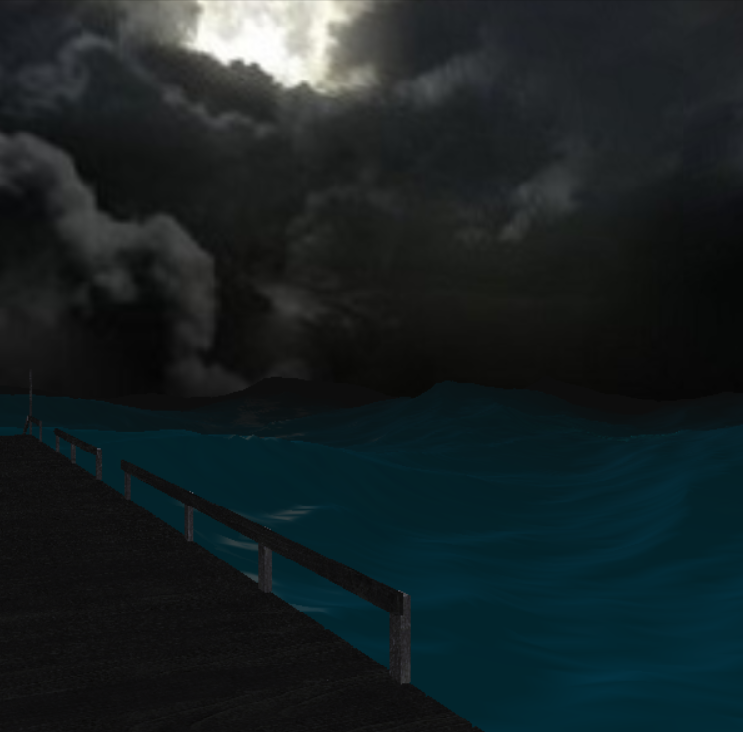
\includegraphics{images/render1.png}
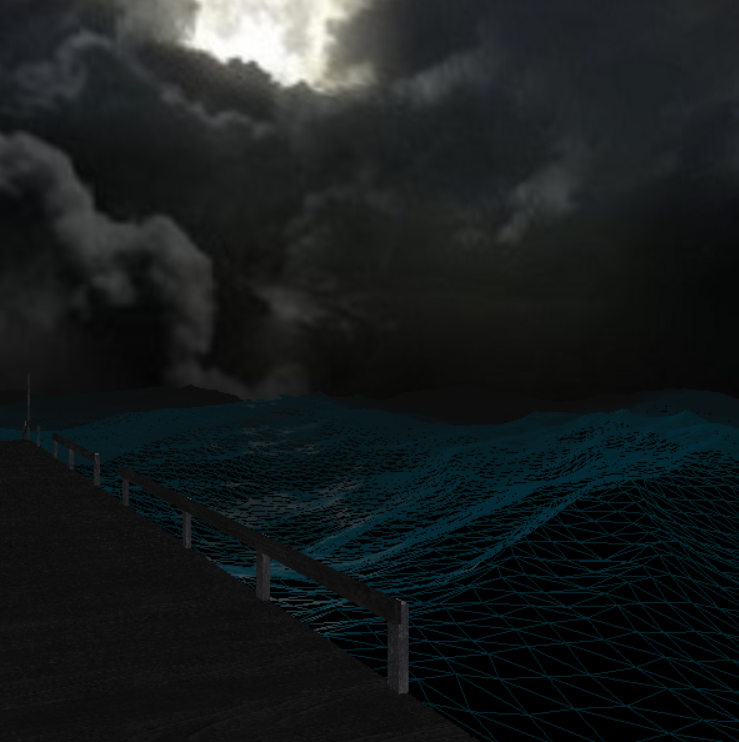
\includegraphics{images/render2.png}
\\

\par The program can be built using the submitted files and run to see the real time animation allowed by the FFT implementation, however
it requires an OpenGL version not guaranteed by integrated graphics cards, so compatibility issues in running may arise. The program uses the 
glm math library and the SOIL image library. GLM is header-only, and thus very portable, however to compile with SOIL you must download and
build SOIL from source on your machine.
To install the SOIL library in a Ubuntu environment, simply enter
\begin{lstlisting}[language = bash]
$sudo apt-get install libsoil-dev
\end{lstlisting}
in a terminal. (Omit the \$!).\\
For other non-Windows environments, you will have to download the entire source file and
use the makefile they provided to build the library, and place it wherever your system libraries
can be accessed. The makefile provided with my project links to it as -lSOIL.
\par For Windows systems, the \textit{Windows} directory contains a Visual Studio 2015 project for the program.

\par A video file of the program at runtime has been included, it is called \textit{fftOceanRender.mp4}.

\section*{Results and Notes}

The FFT implementation did indeed produce a realistic graphical simulation of ocean waves, as desired. Future improvements would involve offloading more of the computational work to the GPU, more realistic calculation of reflection/refraction of light, and integration into a more complex application, such as a game or simulation.
\end{document}
